\documentclass[border=6pt]{standalone}
\usepackage{tikz}
\usetikzlibrary{positioning}

% Colours approximating the original figure
\definecolor{intfill}{RGB}{233,211,122}    % gold (internal nodes)
\definecolor{leaffill}{RGB}{200,216,242}   % light blue (external/leaf nodes)
\definecolor{nodeline}{RGB}{60,72,140}     % navy
\definecolor{numcol}{RGB}{200,40,40}       % red inorder numbers

\begin{document}
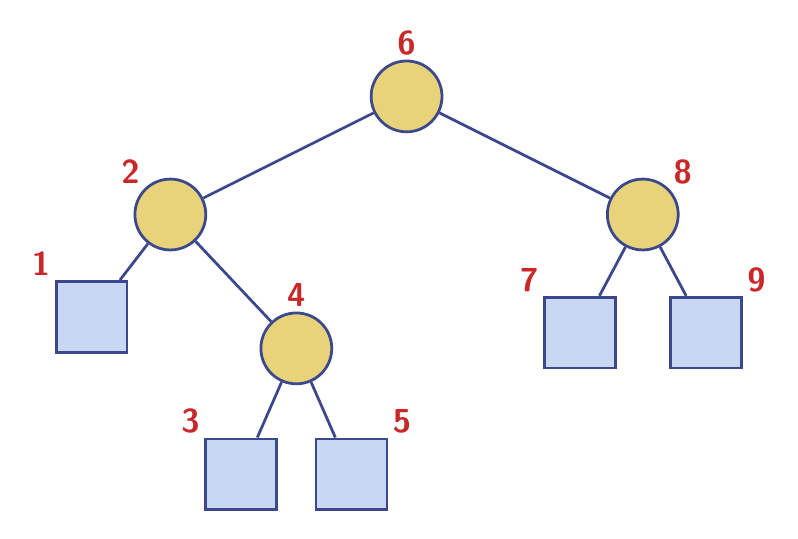
\begin{tikzpicture}[
  font=\sffamily,
  inode/.style={                            % internal node: gold circle
    draw=nodeline, line width=1pt, fill=intfill,
    circle, minimum size=9mm, inner sep=0pt
  },
  leaf/.style={                             % external node: light-blue square
    draw=nodeline, line width=1pt, fill=leaffill,
    rectangle, minimum size=9mm, inner sep=0pt
  },
  num/.style={
    draw=none, fill=none, text=numcol, font=\sffamily\bfseries\large,
    inner sep=1.5pt
  },
  edge/.style={draw=nodeline, line width=1pt},
]

% ---- Nodes (inorder visit number as a coloured label) ----
\node (n6)  at (4.0, 0.6)  [inode, label={[num]above:6}]       {};

\node (n2)  at (1.0,-0.9)  [inode, label={[num]above left:2}]  {};
\node (n8)  at (7.0,-0.9)  [inode, label={[num]above right:8}] {};

\node (l1)  at (0.0,-2.2)  [leaf,  label={[num]above left:1}]  {};
\node (n4)  at (2.6,-2.6)  [inode, label={[num]above:4}]       {};
\node (l7)  at (6.2,-2.4)  [leaf,  label={[num]above left:7}]  {};
\node (l9)  at (7.8,-2.4)  [leaf,  label={[num]above right:9}] {};

\node (l3)  at (1.9,-4.2)  [leaf,  label={[num]above left:3}]  {};
\node (l5)  at (3.3,-4.2)  [leaf,  label={[num]above right:5}] {};

% ---- Edges ----
\foreach \p/\c in {n6/n2, n6/n8,
                   n2/l1, n2/n4,
                   n4/l3, n4/l5,
                   n8/l7, n8/l9}
  \draw[edge] (\p) -- (\c);

\end{tikzpicture}
\end{document}
